\documentclass[../ECON-281-Notes.tex]{subfiles}
\begin{document}
\chapter{Cost Curves}
We will only talk about Short-Run and Long-Run Cost Curves
\section{Short-Run Cost Curves}
In the short run the input variable capital \(K\) is fixed while labour \(L\) is variable.

\begin{Definition}
    {Total Cost}
    The Total cost is comprised with two terms
    \begin{enumerate}
        \item Total Fixed Cost - TFC
        \item Total Variable Cost - TVC
    \end{enumerate}

    \begin{equation}
        TC = TFC + TVC  
    \end{equation}
    You can get the average by dividing all terms with \(Q\).
\end{Definition}

\begin{DndSidebar}[color=PhbLightGreen]{SR Iso-Cost}
  The short run iso-cost is similar to the long-run iso-cost but the capital $K$ is fixed so we denote this with $\overline{K}$.

  \begin{equation}
    STC = w \times L + r\times \overline{K}
  \end{equation}
  
  The first term $w\times L$ is the \emph{Total Variable Cost} and the second term $r\times \overline{K}$ is the \emph{Total Fixed Cost}.
\end{DndSidebar}


\begin{equation}
    MC = \frac{\Delta TC}{\Delta Q}
\end{equation}

Graphing out the different cost measurements shows us \cref{fig:SR_costs}.
As quantity increases, average fixed costs decreases to 0, and the distance between Average Variable Cost and Average Total Cost gets smaller and smaller as \(Q\) increases.

The \textbf{Marginal Cost} will intersect both the Average Total Cost and Average Variable Cost at their global minimum, as shown by point \(A\) and \(B\). 

The cost curves are opposite images for the production curves. These curves take that shape because of the \emph{law of diminishing return} and \emph{law of diminishing marginal product}. As productivity increases cost decrease, and as productivity decreases cost increases. 

In the short-run firms are forced to use a level of capital that may not be optimal. In \cref{fig:SR_inflex} the best bundle to produce \(Q_2\) is bundle B but if \(K\) is fixed at \(K_1\) the firm is forced to use bundle C to produce \(Q_2\) which is not the optimal bundle. Due to the short run input inflexibility the firm may not produce with the lowest cost which is not the case in the long run. 
\begin{figure}[!h]
    \centering
    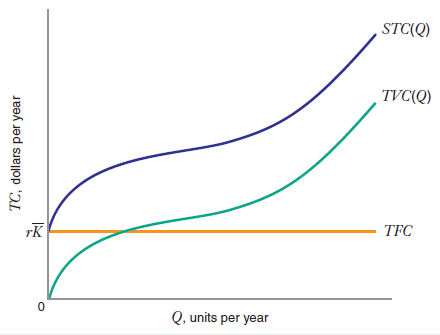
\includegraphics[width=\columnwidth]{../assets/SRTC.png}   
    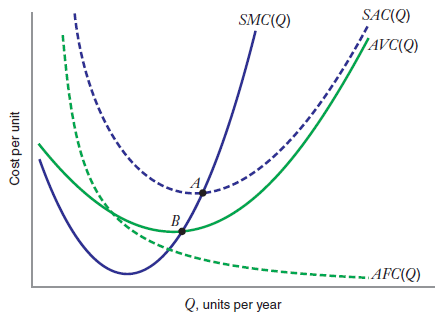
\includegraphics[width=\columnwidth]{../assets/SRMAC.png}   
    \caption{Short-Run Costs}
    \label{fig:SR_costs}
\end{figure}
\begin{figure}[!h]
    \centering
    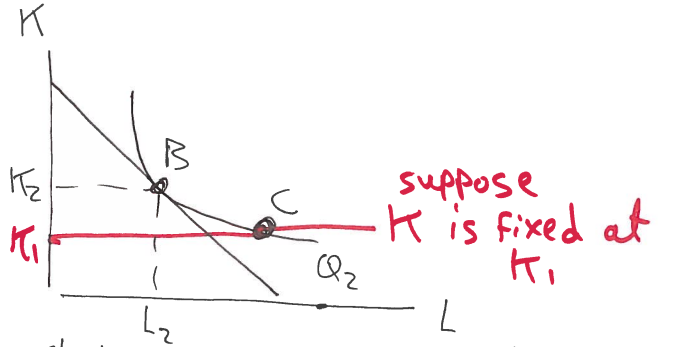
\includegraphics[width=\columnwidth]{../assets/SR_inflex.png}   
    \caption{Short-Run Inflexibility}
    \label{fig:SR_inflex}
\end{figure}

\newpage
~
\newpage

\section{Long-Run Cost Curves}
In the long run both Labour \(L\) and Capital \(K\) are variable. Therefore there are no fixed cost and the total cost \(TC\) is just the Total Variable Cost \(TVC\).

As shown in \cref{fig:LRTC} the Long Run Average Total Cost equals the Long Run Average Variable Cost. The Marginal Cost intersects the Long Run Average Cost at it's global  minima. 
\begin{figure}[h]
    \centering
    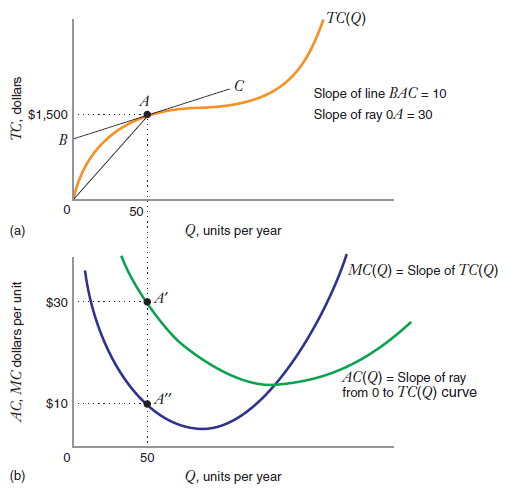
\includegraphics[width=\columnwidth]{../assets/LRTC.png}   
    \caption{Long-Run Total Costs}
    \label{fig:LRTC}
\end{figure}

The Long-Run Average Total Cost \cref{fig:LRAC} is the composition of all the lower envelopes of all short-run ATC curves. The LATC shows the lowest cost of producing every quantity because in the long-run the producer could change and adjust all his inputs and pick the input bundle that produces what he wants with the lowest cost. 
\begin{figure}[h]
    \centering
    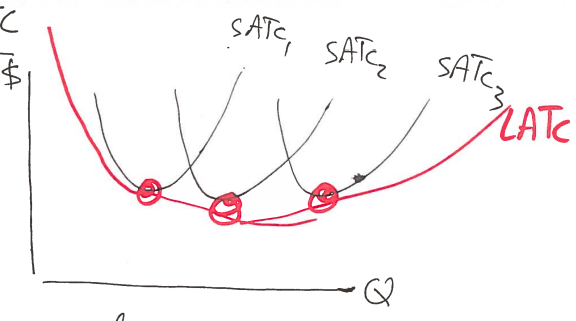
\includegraphics[width=\columnwidth]{../assets/LRAC-0.png}   
    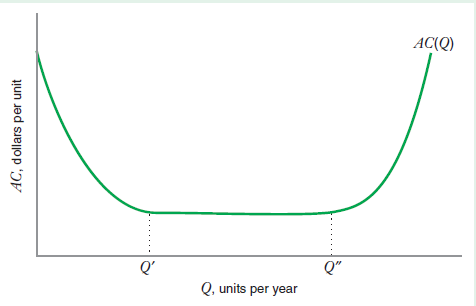
\includegraphics[width=\columnwidth]{../assets/LRAC.png}   
    \caption{Long-Run Average Cost}
    \label{fig:LRAC}
\end{figure}

\subsection{Economics of Scale}
There are three "classes" of Economics of Scales
\begin{enumerate}
    \item Economics of scales is where as \(Q\) increases \(LATC\) decreases between the region \(0\) to \(Q^\prime\).
    \item Efficient scale is where LATC reaches its minimum between the region \(Q^\prime\) and \(Q^{\prime \prime}\).
    \item Diseconomies of scale is where as \(Q\) increases \(LATC\) also increases between the region \(Q^{\prime \prime}\) and beyond. 
\end{enumerate}

\subsection{Output Elasticity of Total Cost \(\varepsilon_{TC,Q}\)}
This measure how responsive TC is to the change in output.
\begin{equation}
    \varepsilon_{TC,Q} = \frac{\%\Delta TC}{\% \Delta Q} = \frac{\Delta TC}{\Delta Q} \times \frac{Q}{TC} = \frac{MC}{ATC} 
\end{equation}


\begin{figure}[h]
    \centering
    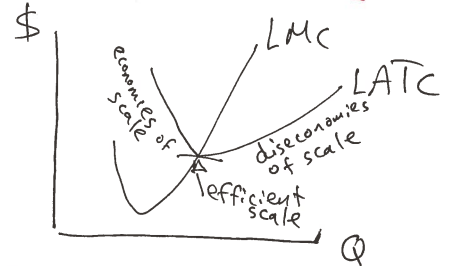
\includegraphics[width=\columnwidth]{../assets/LR_RTS.png}   
    \caption{LATC vs LMC}
    \label{fig:LATC_LMC}
\end{figure}

\begin{itemize}
    \item \(LATC > LMC\) increasing RTS or economics of scale \(\varepsilon_{TC,Q} < 1\)
    \item \(LATC = LMC\) constant RTS or efficient scale \(\varepsilon_{TC,Q} = 1\)
    \item \(LATC < LMC\) decreasing RTS or diseconomies of scale \(\varepsilon_{TC,Q} > 1\)
\end{itemize}

\end{document}
